\documentclass[twocolumn]{article}
\usepackage[utf8]{inputenc}
\usepackage{abstract}
\usepackage{graphicx}
\usepackage{amsmath, amssymb}
\usepackage{hyperref}
\usepackage{caption}
\usepackage{subcaption}
\usepackage{geometry}
\usepackage{booktabs}
\usepackage{float}
\usepackage[backend=biber, style=apa]{biblatex}
\DeclareLanguageMapping{english}{english-apa}
\addbibresource{~/Documents/Zotero/references.bib}
\geometry{margin=1in}

\title{Using Logistic Regression and XGBoost for Bot Detection}
\author{
 Elias Schlie \\
 u783766 \\
 Tilburg University \\
  \texttt{e.p.schlie@tilburguniversity.edu}
}
\date{}

\begin{document}


\twocolumn[
  \maketitle

  \begin{abstract}
 The activity of bots on social media platforms is increasingly becoming a problem and platform providers are seeking ways to prevent bots from infiltrating their systems.
The following project evaluates two simple machine learning algorithms on their ability to discern between bots and users based on their usage data. 
The algorithms applied are logistic regression, which was able to reach an accuracy of $97\%$, and XGBoost, which reached $98\%$ accuracy.
  \end{abstract}
  \vspace{3em}
]

\section{Introduction}

With the rise of large language models, bots now have the ability to immitate human behavior better than ever before. This makes descerning them from actual users increasingly hard, and more sophisticated methods are needed to detect them.

% Describe models

\section{Data and Preprocessing}
% Describe the dataset, relevant features, and how you prepared/split the data.

\subsection{Dataset Description}

The 
"bots\_vs\_users.csv" dataset contains information on $5874$ social media accounts, exactly half of which are bots. Every account has $59$ features, that include $14$ numerical ones like their \texttt{average\_views} and $45$ categorical ones like the city they live in. $41$ of the categorical features are binary like the the variable \texttt{has\_profile\_picture} for example.
Most of the features include a large number of missing or unknown values. 4483 accounts don't contain any numerical information, while for the individual categorical features, between 5006 and 24 of the accounts cary the label "unknown".
Only the target varialbe "target", which indicates if the account is a bot or not has no missing features.

\subsection{Data split}

Before any preprocessing was applied, the data was split into a training and a test set using a stratified 80/20 split. This was done prior to preprocessing due to the reason that some of the preprocessing steps learn from the data and thus would lead to data leakage if applied to the entire dataset at once. Model hyperparameters were validated based on a k-fold cross validation on the training set. To ensure reproducibility, this and every following step that involves randomness was seeded with the seed $42$.

\subsection{Preprocessing and Feature Engineering}

All the preprocessing and feature engineering steps were implemented in a single \texttt{DataCleaner} class. The class's \texttt{fit\_transform} method was used on the training data and transforms it while learning distributional features from it for functions like scaling. The \texttt{transform} method applies the same transformations with the previously learned features and was used on the testing dataset. This sections lists all the transformations in the order they were applied.

\paragraph{Minimal profile flag}
A binary categorical feature was added, descerning between the accounts that have numeric features and the accounts without them. This step was done first because later steps add further numeric variables, which have missing values for different users, but the intended variable was intended to capture exactly the set of users that don't have numeric features in the initial dataset.

\paragraph{Subscribers Count Feature}
While reflecting a numeric quantity, the \texttt{subscribers\_count} feature was stored as a categorical variable with $1597$ possible categories. To enable the machine learning algorithms, to learn from the numeric relationships, this variable was converted to be numeric.

\paragraph{Data Scaling}
To ensure equal contribution of features and faster convergence for the logistic regressor, the data was scaled with the \texttt{StandarScaler} of the \texttt{sklearn} python library.

\paragraph{Median imputation}
The \texttt{SimpleImputer} class of the \texttt{sklearn} library was used to replace all missing values for numerical features with the median of this feature. That way, it is possible for the logistic regressor to use the numeric features without creating unnecessary noise. 

\paragraph{Categorical encoding}
Categorical features with exactly two categories were binary encoded, mapping each category to 0 or 1. The remaining categories were one-hot encoded, while assigning all categories with less than 30 members into an \texttt{other} bin. This \texttt{other} bin had the effect of reducing the number of city categories from 362 to only 6 and thereby preventing a drastic dimensionality increase that would have otherwise come from one-hot encoding it. For all categorical features, the \texttt{unknown} category was treated just as any other category.

\section{Models}

\subsection{Baseline}

For a baseline measurement, \texttt{sklearn}'s \texttt{DummyClassifier} was used with the "stratified" stragety. This strategy randomly predicts labels based on the frequency with which they occur in the dataset. It achieved an accuracy of 0.5 and an F1-score of 0.49 on the bot class.

\subsection{Logistic Regressor}

Logistic regression is one of the simplest machine learning algorithms. Despite its simplicity, it performs surprisingly well on linearly separable classification tasks. A major advantage of logistic regression is that its coefficients directly reflect feature importance for the classification task and can thus easily be interpreted. Additionally, it is very computationally efficient when dealing with large feature spaces. This makes it a good choice for local hyperparameter tuning and evaluation on the current dataset.

\subsection{XGBoost}

XGBoost (Extreme Gradient Boosting) is a high-performance implementation of gradient-boosted decision trees designed for speed and efficiency. \parencite{chenXGBoostScalableTree2016} As other decision tree derived algorithms, it is particularly well-suited for structured datasets with a mix of categorical and numerical features, as in the current case.

\subsection{Model Comparison}

The most striking difference between logistic regression and XGBoost is their ability to handle non-linear data. While XGBoost can pick up on complex non-linear relationships, logistic regression doesn't have this ability. 
Next to this difference, the two algorithms are similar in that they both are very compute efficient and use regularization to decrease overfitting, which is essential when working with high dimensional data.

\section{Model Training}

\subsection{Logistic Regression}

A critical hyperparameter in logistic regression is \texttt{C}, which controls the strength of regularization. Lower \texttt{C} values impose stronger regularization, shrinking the model's coefficients toward zero (in the case of the default L2 penalty), and thereby reducing the risk of overfitting.

A grid search was performed using \texttt{GridSearchCV} from \texttt{scikit-learn} to select the optimal regularization parameter \texttt{C}, testing the values 0.01, 0.1, 0.25, 0.5, 1, 2.5, 5, 10, 20, 40, and 80. \texttt{C} = 2.5 was identified as the best value and a model was trained on the whole training set.

As visible in Figure~\ref{fig:c_value_performance} in the appendix, the average F1 score across five folds peaks around the value of 2.5, confirming the value arived at with gridsearch. Nevertheless, the error bars clearly indicate that the effect is extremely small. The difference between the worst and the best mean F1 score is only around 0.004\%, indicating, that regularization strength doesn't have a strong impact on performance in thi dataset.

The final linear regressor was trained on the entire training set with a \texttt{C} value of 2.5.

\subsection{XGBoost}

With way more relevant hyperparameters than logistic regression, leading to a combinatorial explosion, gridsearch proved unsuitable and Optuna \parencite{akibaOptunaNextgenerationHyperparameter2019} was used instead. Optuna is an open-source hyperparameter optimizing framework that can efficiently search through t a large space of possible hyperparameter combinations. It uses advanced strategies like Bayesian optimization to intelligently explore the search space, thereby siginificantly reducing the number of tests that need to be done to arrive at a good result.

To ensure reliabile results, every hyperparameter combination was scored on its average F1 score over 5 independently seeded 3-fold cross-validations. Optuna conducted a total of 100 trials with different combinations of hyperparameters. The best performing configuration achieved an average F1 score of 0.9781. Search ranges for hyperparameters and the resulting best combination can be found in Table~\ref{tab:xgb_best_params}.

\begin{table}[H]
\centering
\caption{Best hyperparameter configuration for XGBoost and corresponding search ranges}
\label{tab:xgb_best_params}
\begin{tabular}{lll}
\toprule
\textbf{Hyperparameter} & \textbf{Best Value} & \textbf{Search Range} \\
\midrule
\texttt{n\_estimators}       & 281     & [50, 500] \\
\texttt{learning\_rate}      & 0.2003  & [0.01, 0.3] \\
\texttt{max\_depth}          & 3       & [3, 8] \\
\texttt{min\_child\_weight}  & 1       & [1, 5] \\
\texttt{subsample}          & 0.9284  & [0.6, 1.0] \\
\texttt{colsample\_bytree}   & 0.6527  & [0.6, 1.0] \\
\texttt{gamma}              & 1.0618  & [0, 5] \\
\bottomrule
\end{tabular}
\end{table}

Like previously with the logistic regressor, variance between the best and worst set of hyperparameters was only minimal, this time spanning a little more than 0.005\% in average F1 performance. Due to the fact that different hyperparameters are interacting, looking at them separately from each other becomes less meaningful and harder to interpret. Figure~\ref{fig:xgboost_hyper_compare} attemps this by visualizing how learning rate and gamma influence F1 score. It reveals, that a learning rate around 0.2 ressults in slightly higher F1 scores while higher gamma values tend to slightly decrease prediction performance.

The final model used a the best parameters listed in Table~\ref{tab:xgb_best_params} collumn two and was re-trained on the entire training set.

\section{Results}

\subsection{Logistic regression}
On the hold-out test set, the logistic regressor reached an F1 score of 0.9724, accuracy of 0.9728, precision of 0.9843, recall of 0.9608, and an area under curve (AUC) for the receiver operating characteristic (ROC) of 0.9951. Table~\ref{tab:log_confusion} displays the confunsion matrix of the predictions, revealing that only 23 out of 587 bots got misclassified as users. A ROC curve and a precision-recall curve can be found in figure~\ref{fig:log_ROC_curve} and figure~\ref{fig:log_precision_recall_curve} of the appendix respectively.

\subsection{XGBoost}
XGBoost was able to achieve an F1 score of 0.9768, accuracy of 0.9770, precision of 0.9861, recall of 0.9676, and ROC-AUC of 0.9962. Those metrics are reflected in it's confusion matrix (Table~\ref{tab:xgb_confusion}) that shows only 19 misclassified bots. Like previously with the logistic regression, the ROC curve (figure~\ref{fig:xgb_ROC_curve}) and a precision-recall curve (figure~\ref{fig:xgb_precision_recall_curve}) are very close to the optimum.

\section{Discussion}

\subsection{Model Performance Comparison}
While XGBoost performs slightly better on all metrics, this difference is extremely small. With only 19 instead of 23 misclassified bots and only 8 instead of 9 misclassified users, XGBoosts accuracy is 0.0042 points higher than the one of logistic regression. This is also reflected in F1 score, where the difference increases slightly to 0.0044 points.
Those differences are incredibly small and clearly show that XGBoosts ability to find non-linear relationships in data is not majorly critical for the given dataset.

\subsection{Generalizability}

Both models seem to generalize extremely well and don't show signs of overfitting to the training data. Comparing the F1 scores during hyperparameter tuning and testing shows only minimal differences of 0.0013 points in the F1 score of XGBoost. This difference is extremely small, especially when considering that hyperparameters were specifically chosen to fit the training set as well as possible.

\subsection{Feature Analysis}

The \texttt{Explainer} class of the python \texttt{shap} library was used to extract SHAP values for the different features. Figures~\ref{fig:log_shap_bar}, \ref{fig:log_shap_bee}, \ref{fig:xgb_shap_bar}, and \ref{fig:xgb_shap_bee} visualize those, showing a high amount of overlap with the six most important features of the logistic regressor all being in the top eigt most important features. Notably, the one hot encoding of the unknown class in the \texttt{has\_status} feature is the most important feature for both algorithms. 
Specifically looking at the gender variable reveals for both algorithms, the error rate decreases with increasing frequency of the category, (Table~\ref{tab:gender_analysis}) resulting in the positive class having the lowest error rate.

\section{Reflection}

Through consistent seeding, the results of this report can easily reproduced. With different seeds, it is not unlikey to arrive at a different combination of hyperparameters because of the small error differences between tests. As shown in Figure~\ref{fig:c_value_performance}, the variability from different splits far exceeded the variability from different \texttt{C} values. Therefore, it's possible that different seeds for splitting the dataset lead to different best \texttt{C}s just by chance. While extensive testing with systematically different split seeds was implemented, which definitely decreased variability in results, XGB different seeds will most likely still result in different sets of hyperparameters.

\printbibliography

\onecolumn
\appendix
\newpage

\section{Tables}
\renewcommand{\thetable}{A.\arabic{table}}
\setcounter{table}{0}

\begin{table}[H]
\centering
\caption{Confusion matrix for logistic regression predictions on the test set}
\label{tab:log_confusion}
\begin{tabular}{lcc}
\toprule
 & \textbf{Predicted Users} & \textbf{Predicted Bots} \\
\midrule
\textbf{Users} & 579 & 9 \\
\textbf{Bots} & 23  & 564 \\
\bottomrule
\end{tabular}
\end{table}

\begin{table}[H]
\centering
\caption{Confusion matrix for XGBoost predictions on the test set}
\label{tab:xgb_confusion}
\begin{tabular}{lcc}
\toprule
 & \textbf{Predicted Users} & \textbf{Predicted Bots} \\
\midrule
\textbf{Users} & 580 & 8 \\
\textbf{Bots} & 19  & 568 \\
\bottomrule
\end{tabular}
\end{table}

\begin{table}[H]
\centering
\caption{Error counts, total samples, and error rates by gender}
\label{tab:gender_analysis}
\begin{tabular}{lrrrrr}
\toprule
 & LR Errors & XGB Errors & Total Members & LR Error Rate & XGB Error Rate \\
gender &  &  &  &  &  \\
\midrule
1.0 & 19 & 17 & 888 & 0.021 & 0.019 \\
2.0 & 12 & 9 & 278 & 0.043 & 0.032 \\
other & 1 & 1 & 9 & 0.111 & 0.111 \\
\bottomrule
\end{tabular}
\end{table}

\vfill

\newpage
\section{Figures}
\renewcommand{\thefigure}{A.\arabic{figure}}
\setcounter{figure}{0}

\begin{figure}[h]
    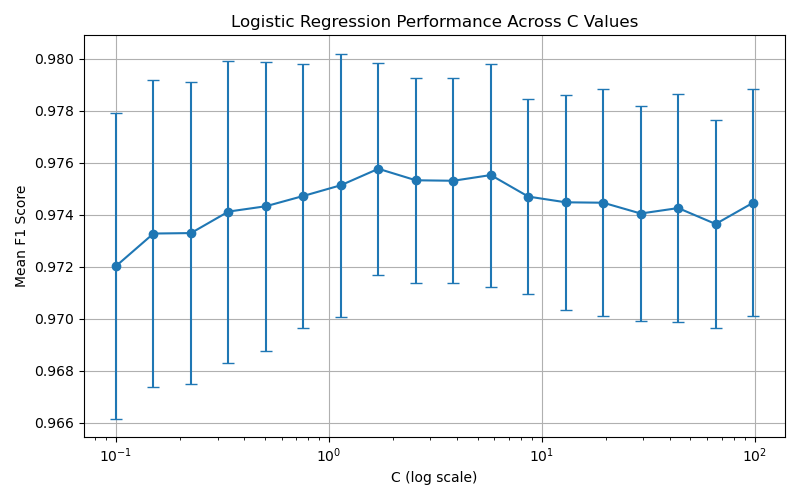
\includegraphics[width=\linewidth]{Figures/Logistic_Regression_Performance_Across_C_Values.png}
    \caption{Mean F1 score of logistic regression across different regularization strengths (C), evaluated using 5-fold stratified cross-validation. Error bars represent the standard deviation across folds. A log scale is used on the x-axis to capture the exponential range of tested C values. While a peak around 2.5 is visible, the error bars suggest that the effect of C is only minimal.}
    \label{fig:c_value_performance}
\end{figure}

\begin{figure}[h]
    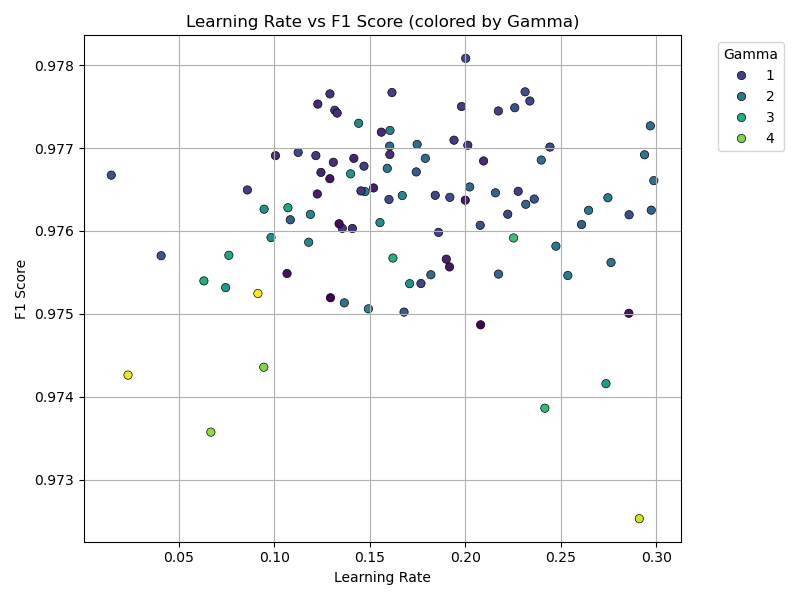
\includegraphics[width=\linewidth]{Figures/Learning_Rate_vs_F1_Score__colored_by_Gamma_.png}
    \caption{Scatterplot of the effect of the XGBoost hyperparameters \texttt{learning\_rate} and \texttt{gamma} on average F1 score.}
    \label{fig:xgboost_hyper_compare}
\end{figure}

\begin{figure}[h]
    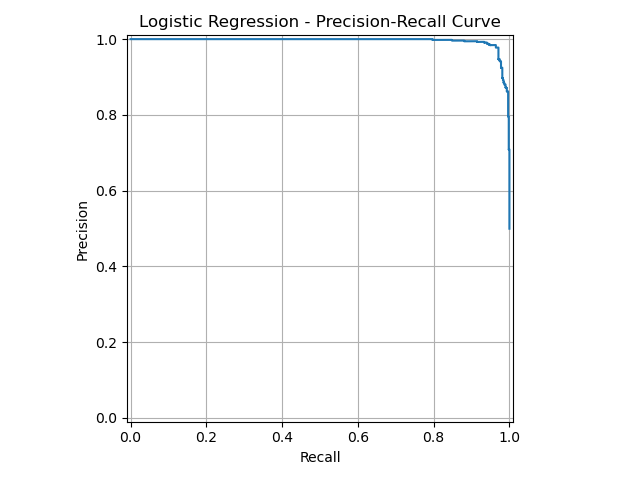
\includegraphics[width=\linewidth]{Figures/Logistic_Regression___Precision_Recall_Curve.png}
    \caption{Precision recall curve of the logistic regressor on the hold-out test set.}
    \label{fig:log_precision_recall_curve}
\end{figure}

\begin{figure}[h]
    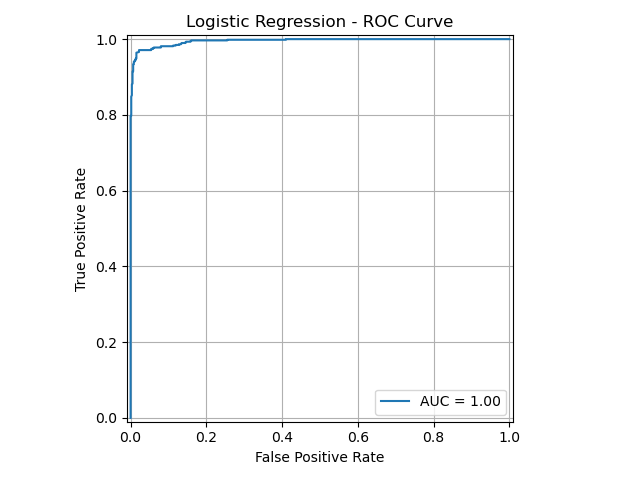
\includegraphics[width=\linewidth]{Figures/Logistic_Regression___ROC_Curve.png}
    \caption{Receiver operating characteristic curve of the logistic regressor on the hold-out test set.}
    \label{fig:log_ROC_curve}
\end{figure}

\begin{figure}[h]
    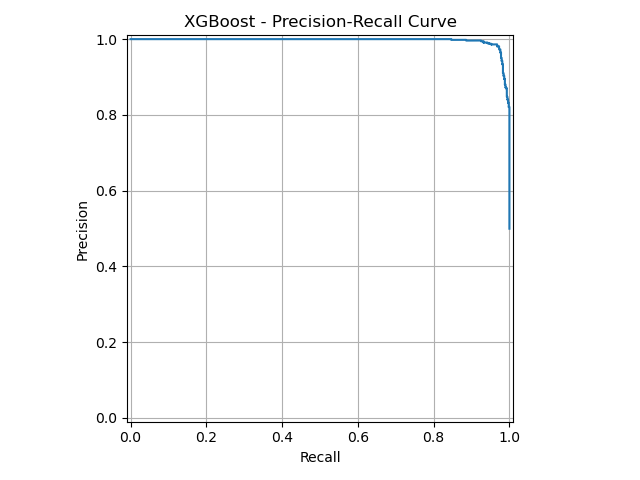
\includegraphics[width=\linewidth]{Figures/XGBoost___Precision_Recall_Curve.png}
    \caption{Precision recall curve of XGBoost on the hold-out test set.}
    \label{fig:xgb_precision_recall_curve}
\end{figure}

\begin{figure}[h]
    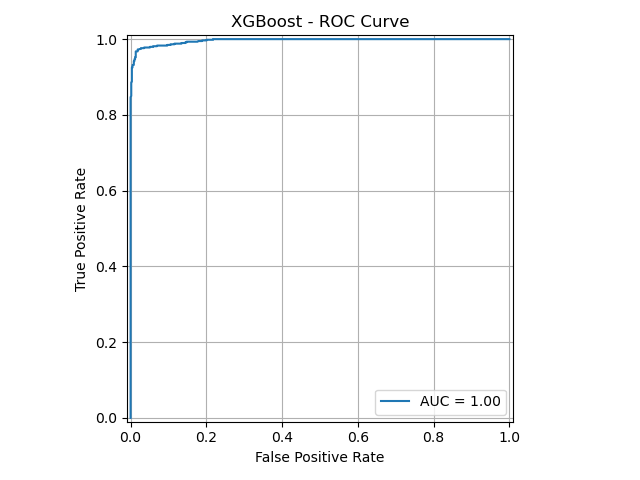
\includegraphics[width=\linewidth]{Figures/XGBoost___ROC_Curve.png}
    \caption{Receiver operating characteristic curve of XGBoost on the hold-out test set.}
    \label{fig:xgb_ROC_curve}
\end{figure}

\begin{figure}[h]
    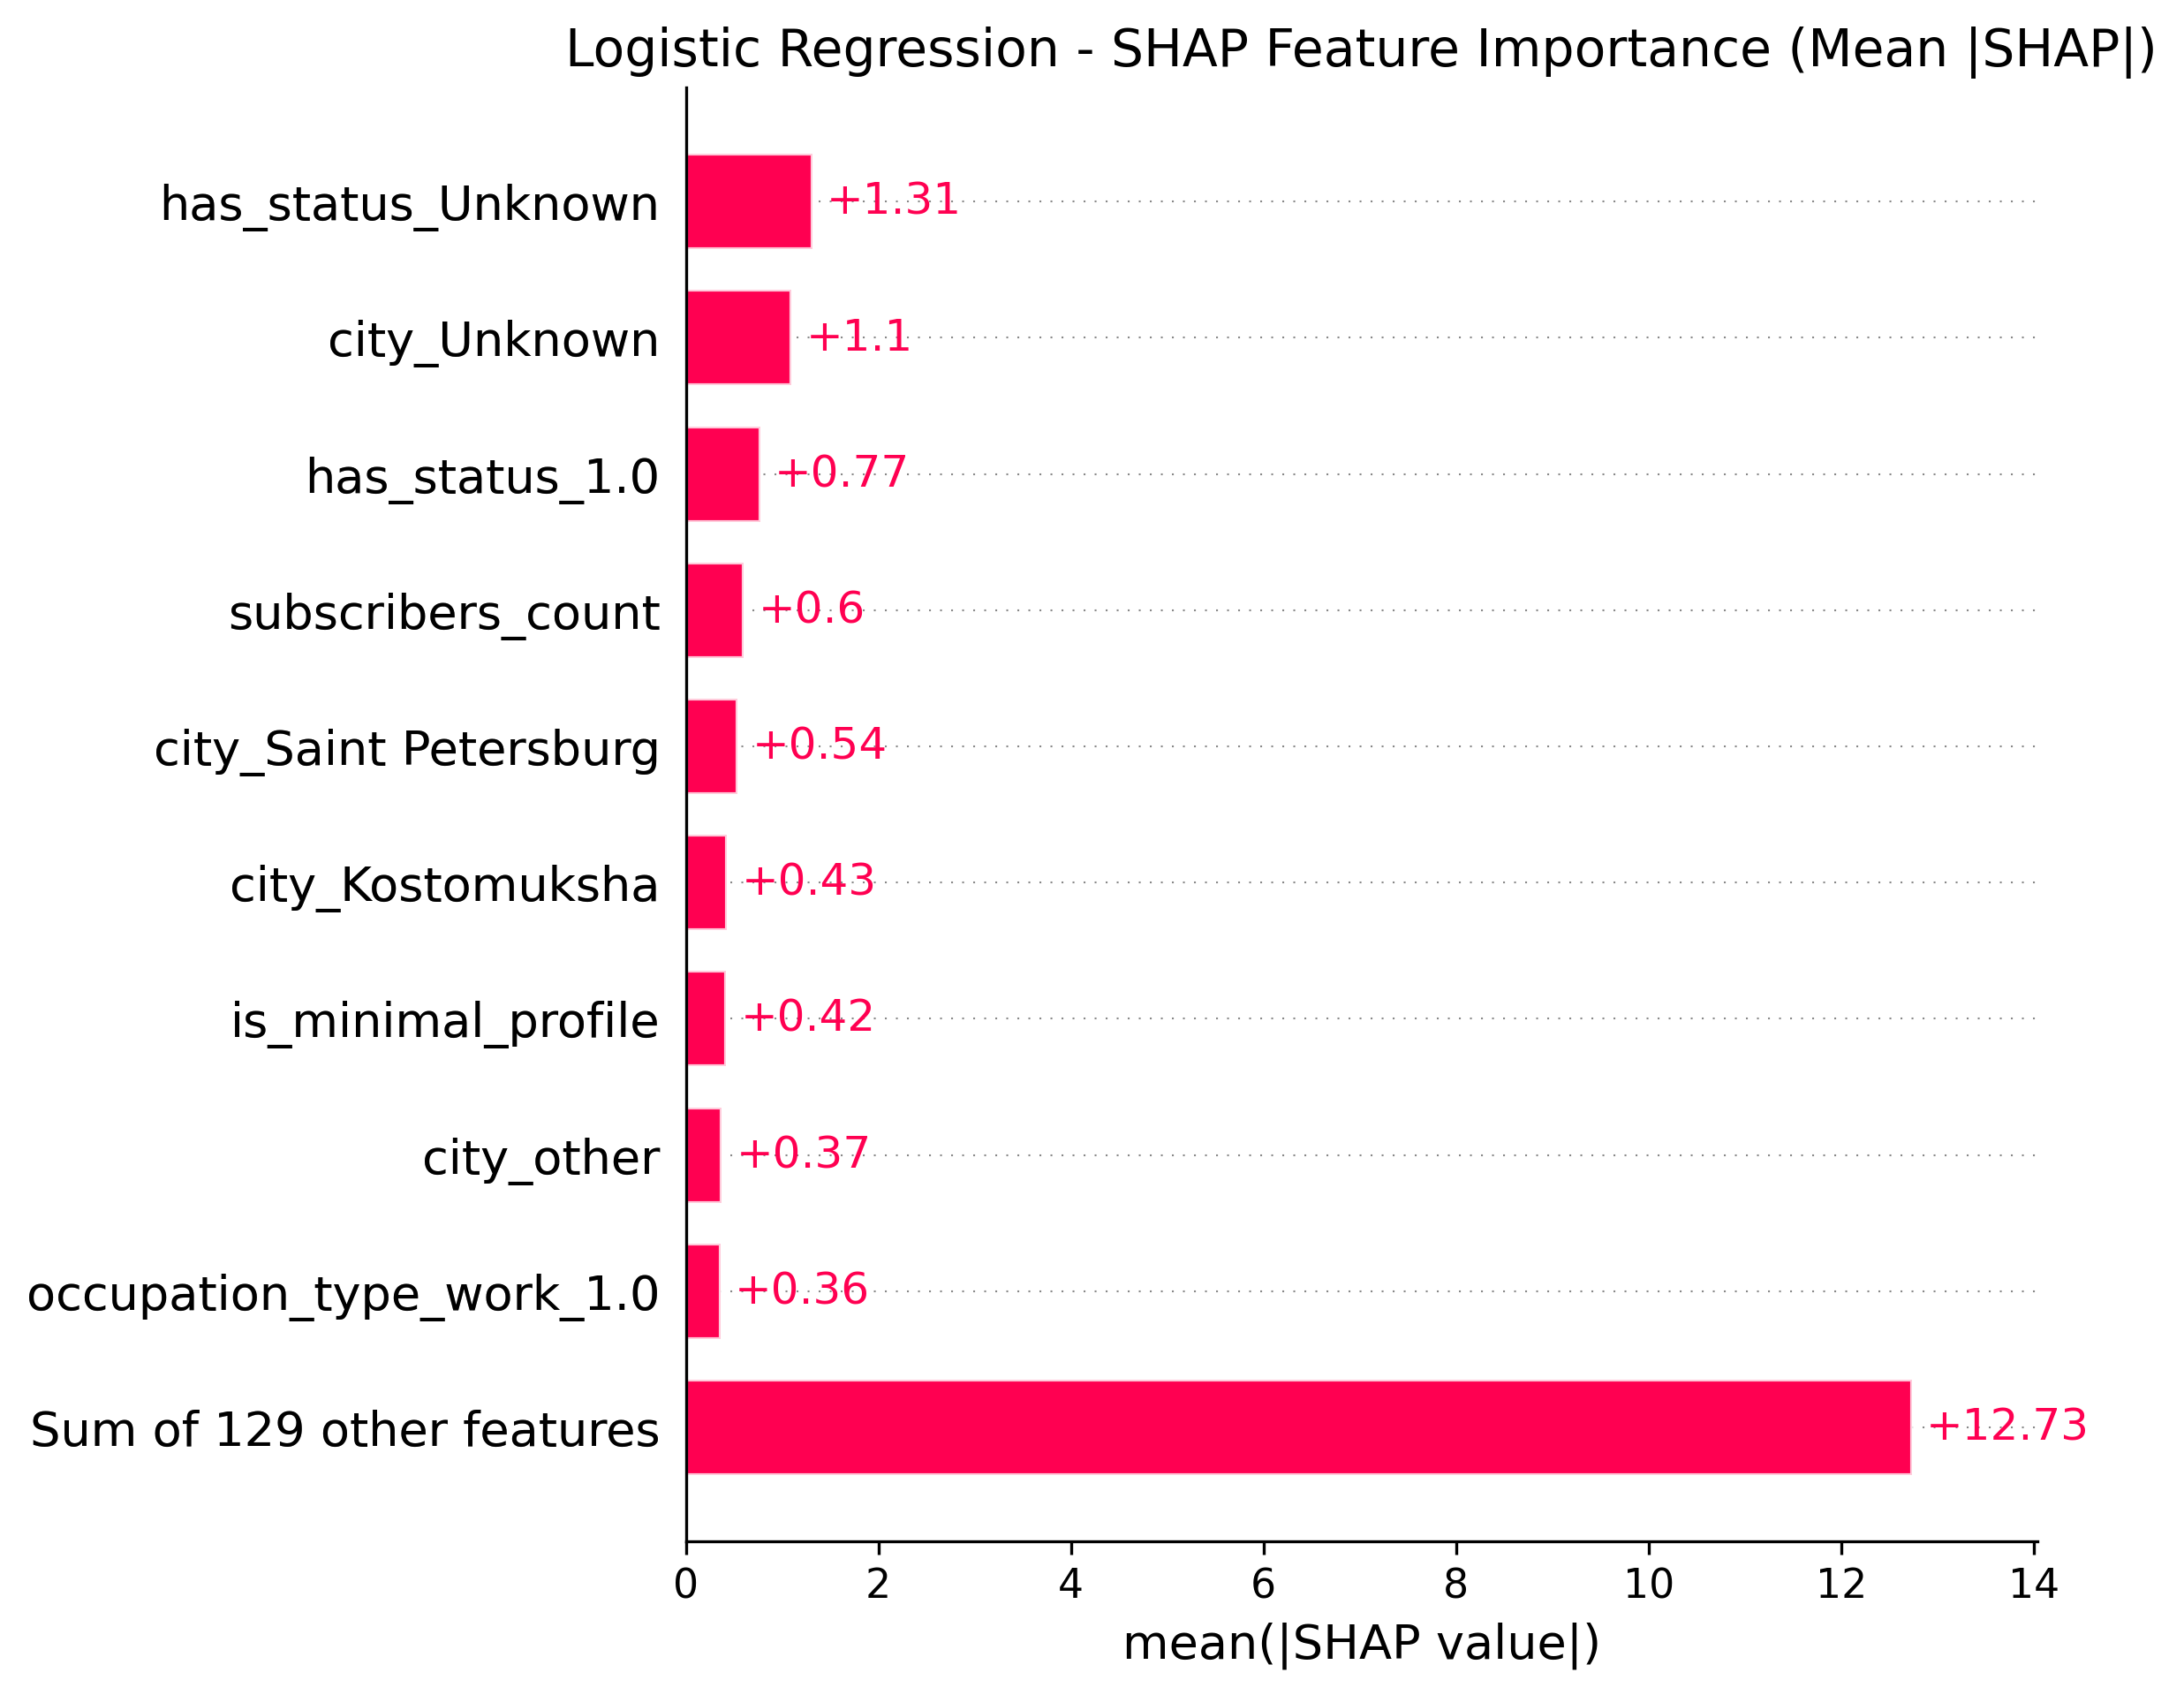
\includegraphics[width=\linewidth]{Figures/shap_bars.png}
    \caption{Bar graph, comparing SHAP feature importance of the 9 most important features in the linear regessor with the summed importance of the 129 remaining features.}
    \label{fig:log_shap_bar}
\end{figure}

\begin{figure}[h]
    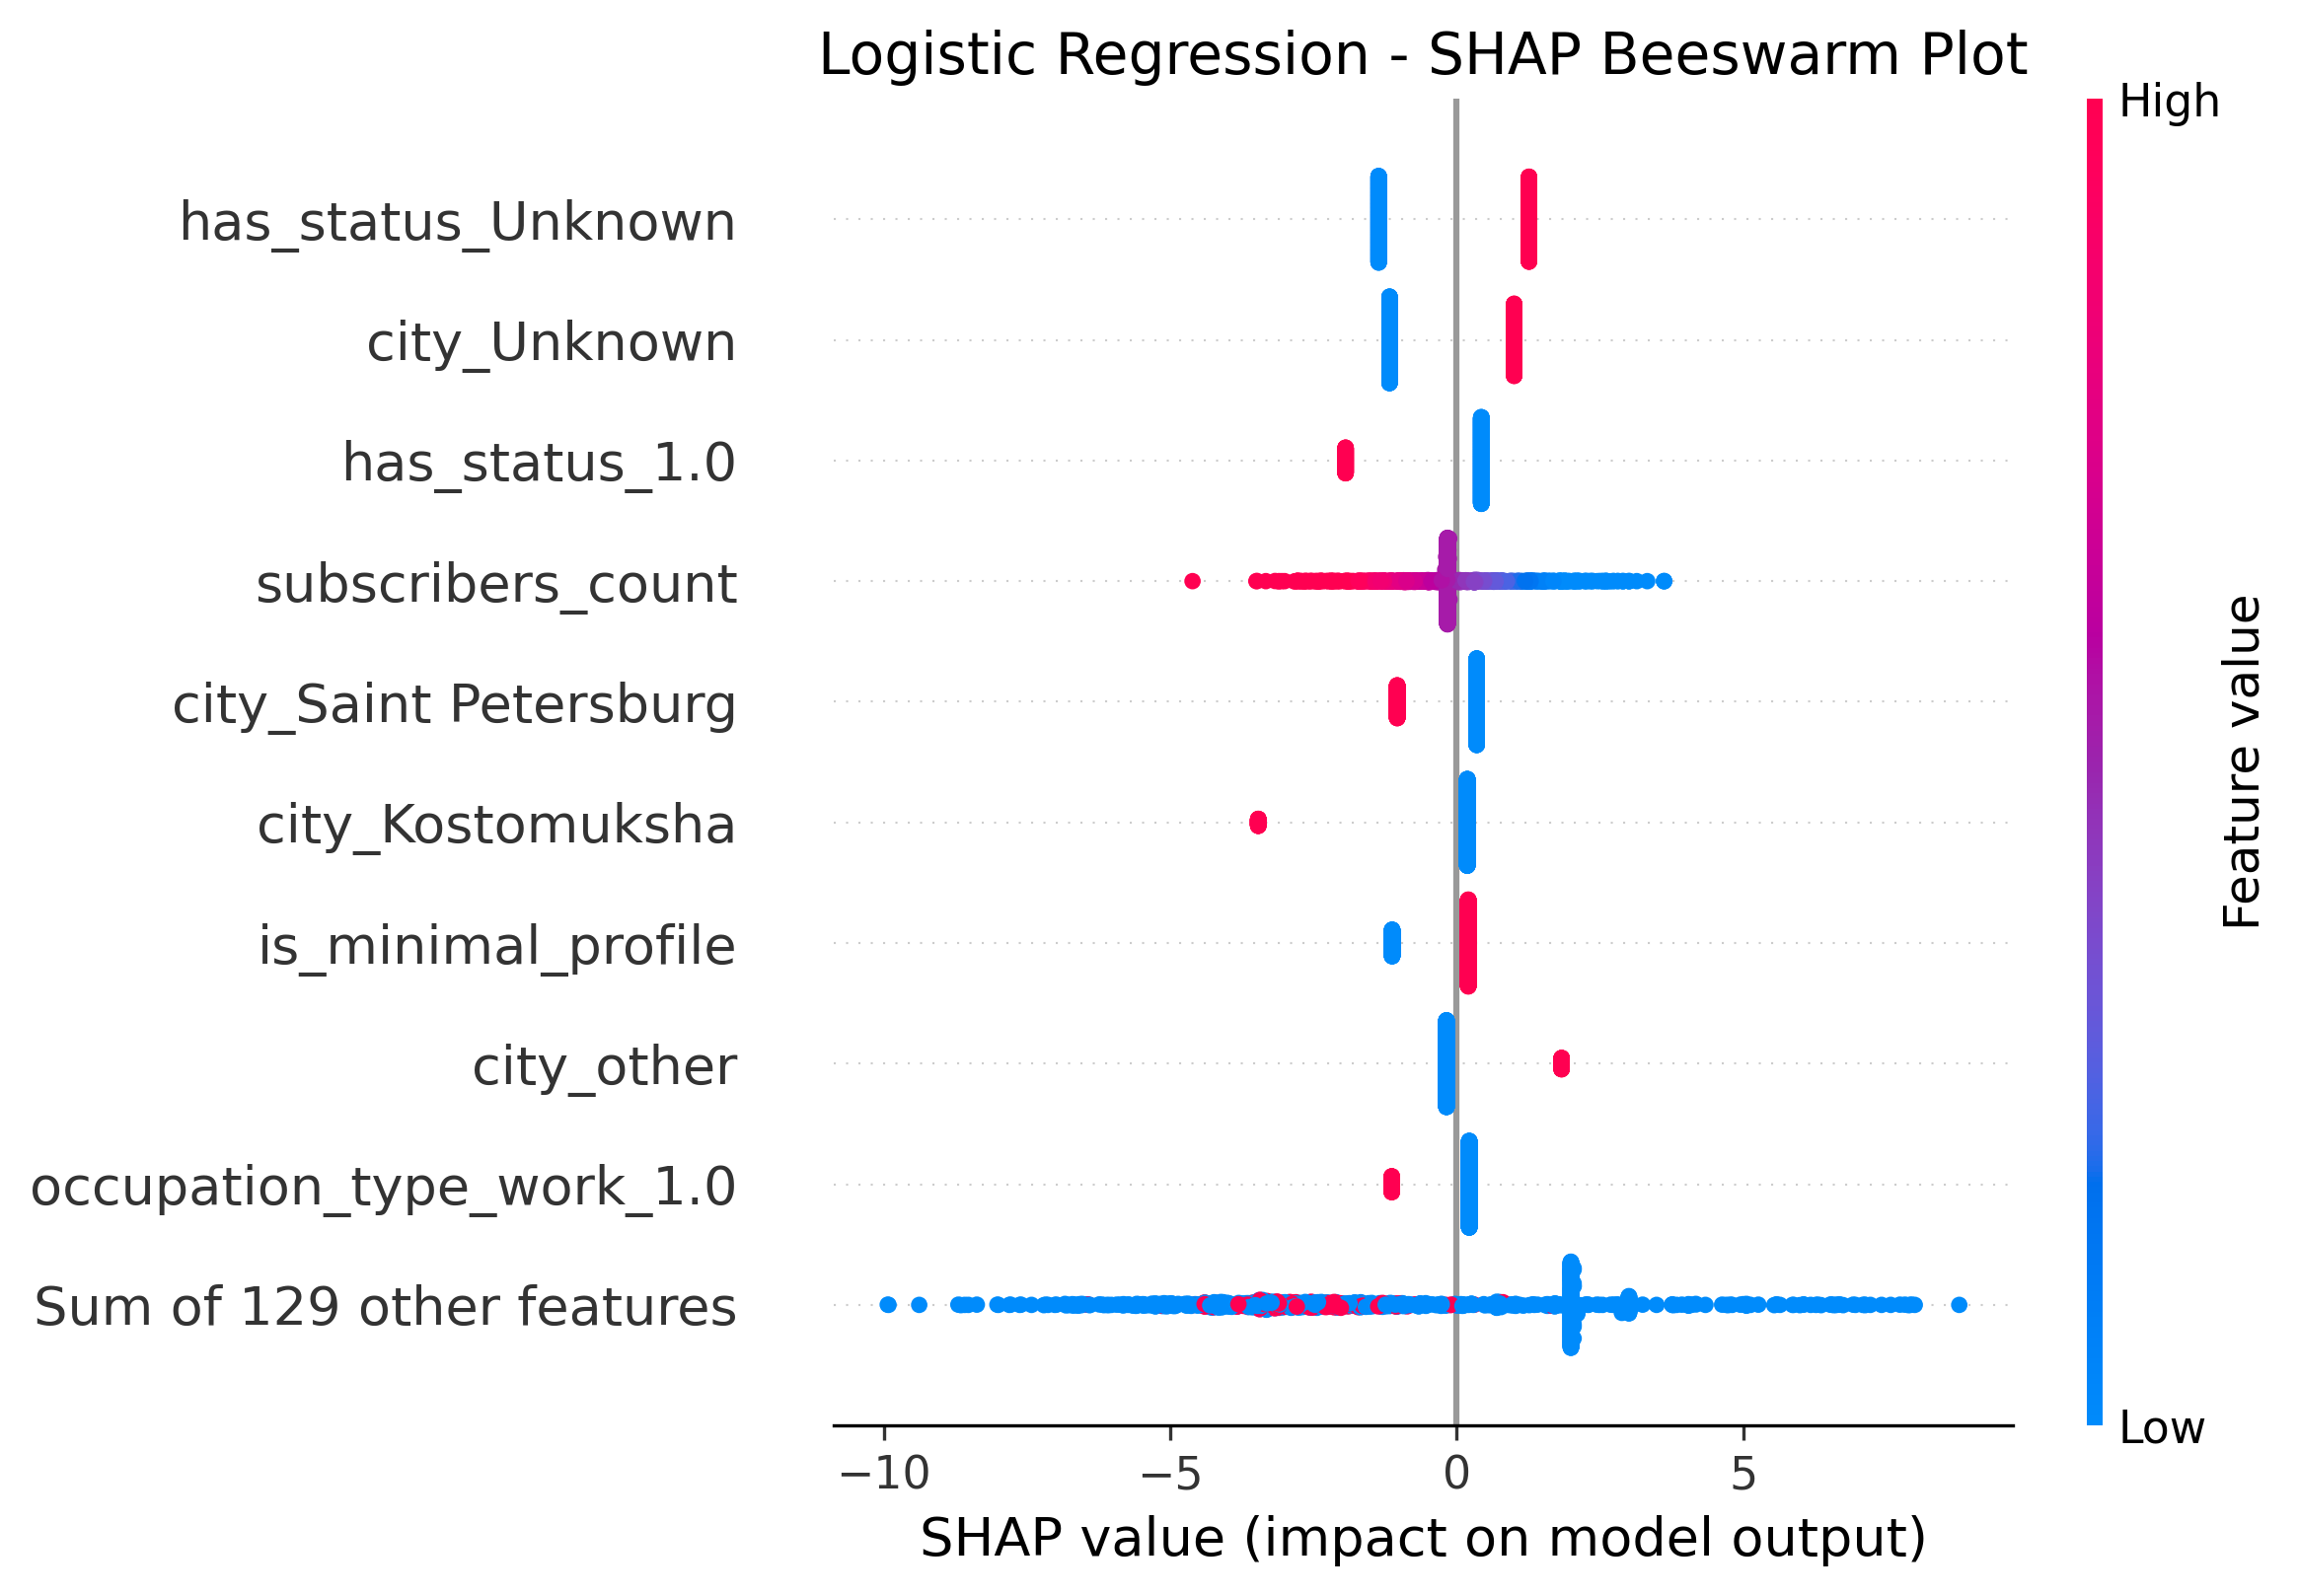
\includegraphics[width=\linewidth]{Figures/shap_beeswarm.png}
    \caption{SHAP beeswarm plot showing the global feature importance for the logistic regressor. Each dot represents a SHAP value for a single prediction and feature. The horizontal position indicates the impact on the model output (positive values push the prediction toward the bot class), while the color reflects the original feature value (red = high, blue = low). Features are sorted top-to-bottom by overall importance.}
    \label{fig:log_shap_bee}
\end{figure}

\begin{figure}[h]
    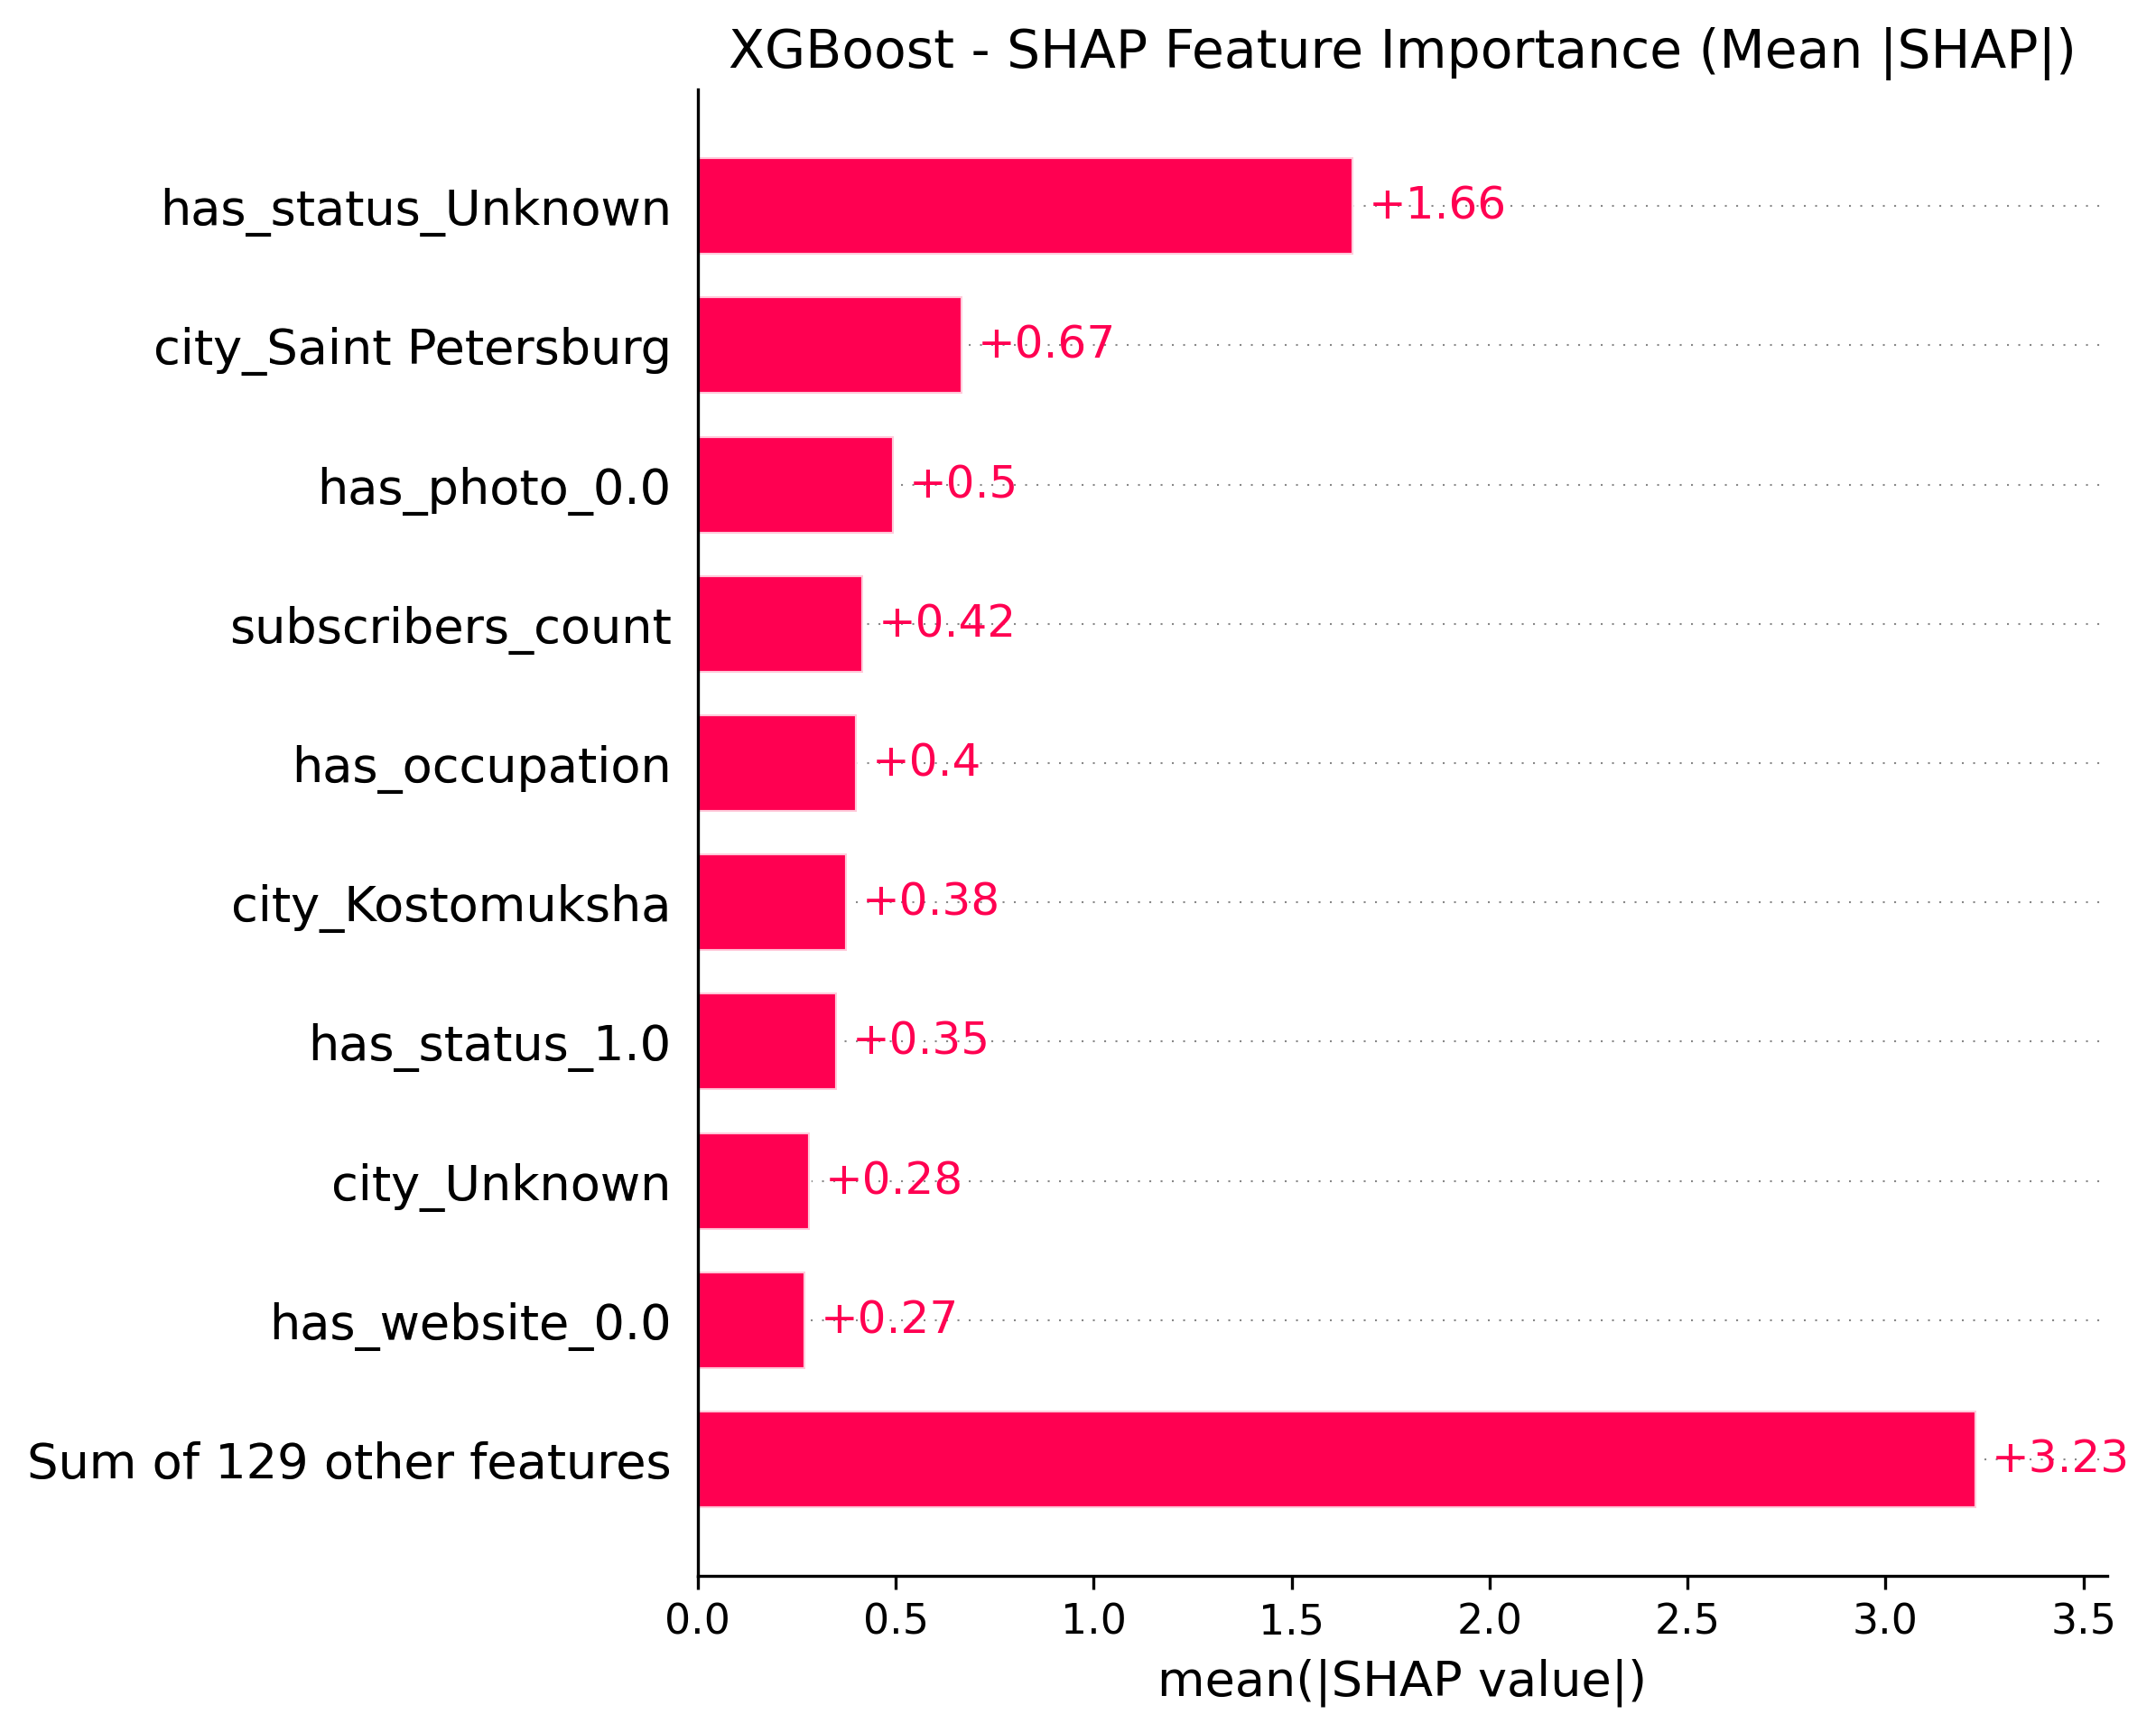
\includegraphics[width=\linewidth]{Figures/xgb_shap_bars.png}
    \caption{Bar graph, comparing SHAP feature importance of the 9 most important features of the trained XGBoost model with the summed importance of the 129 remaining features.}
    \label{fig:xgb_shap_bar}
\end{figure}

\begin{figure}[h]
    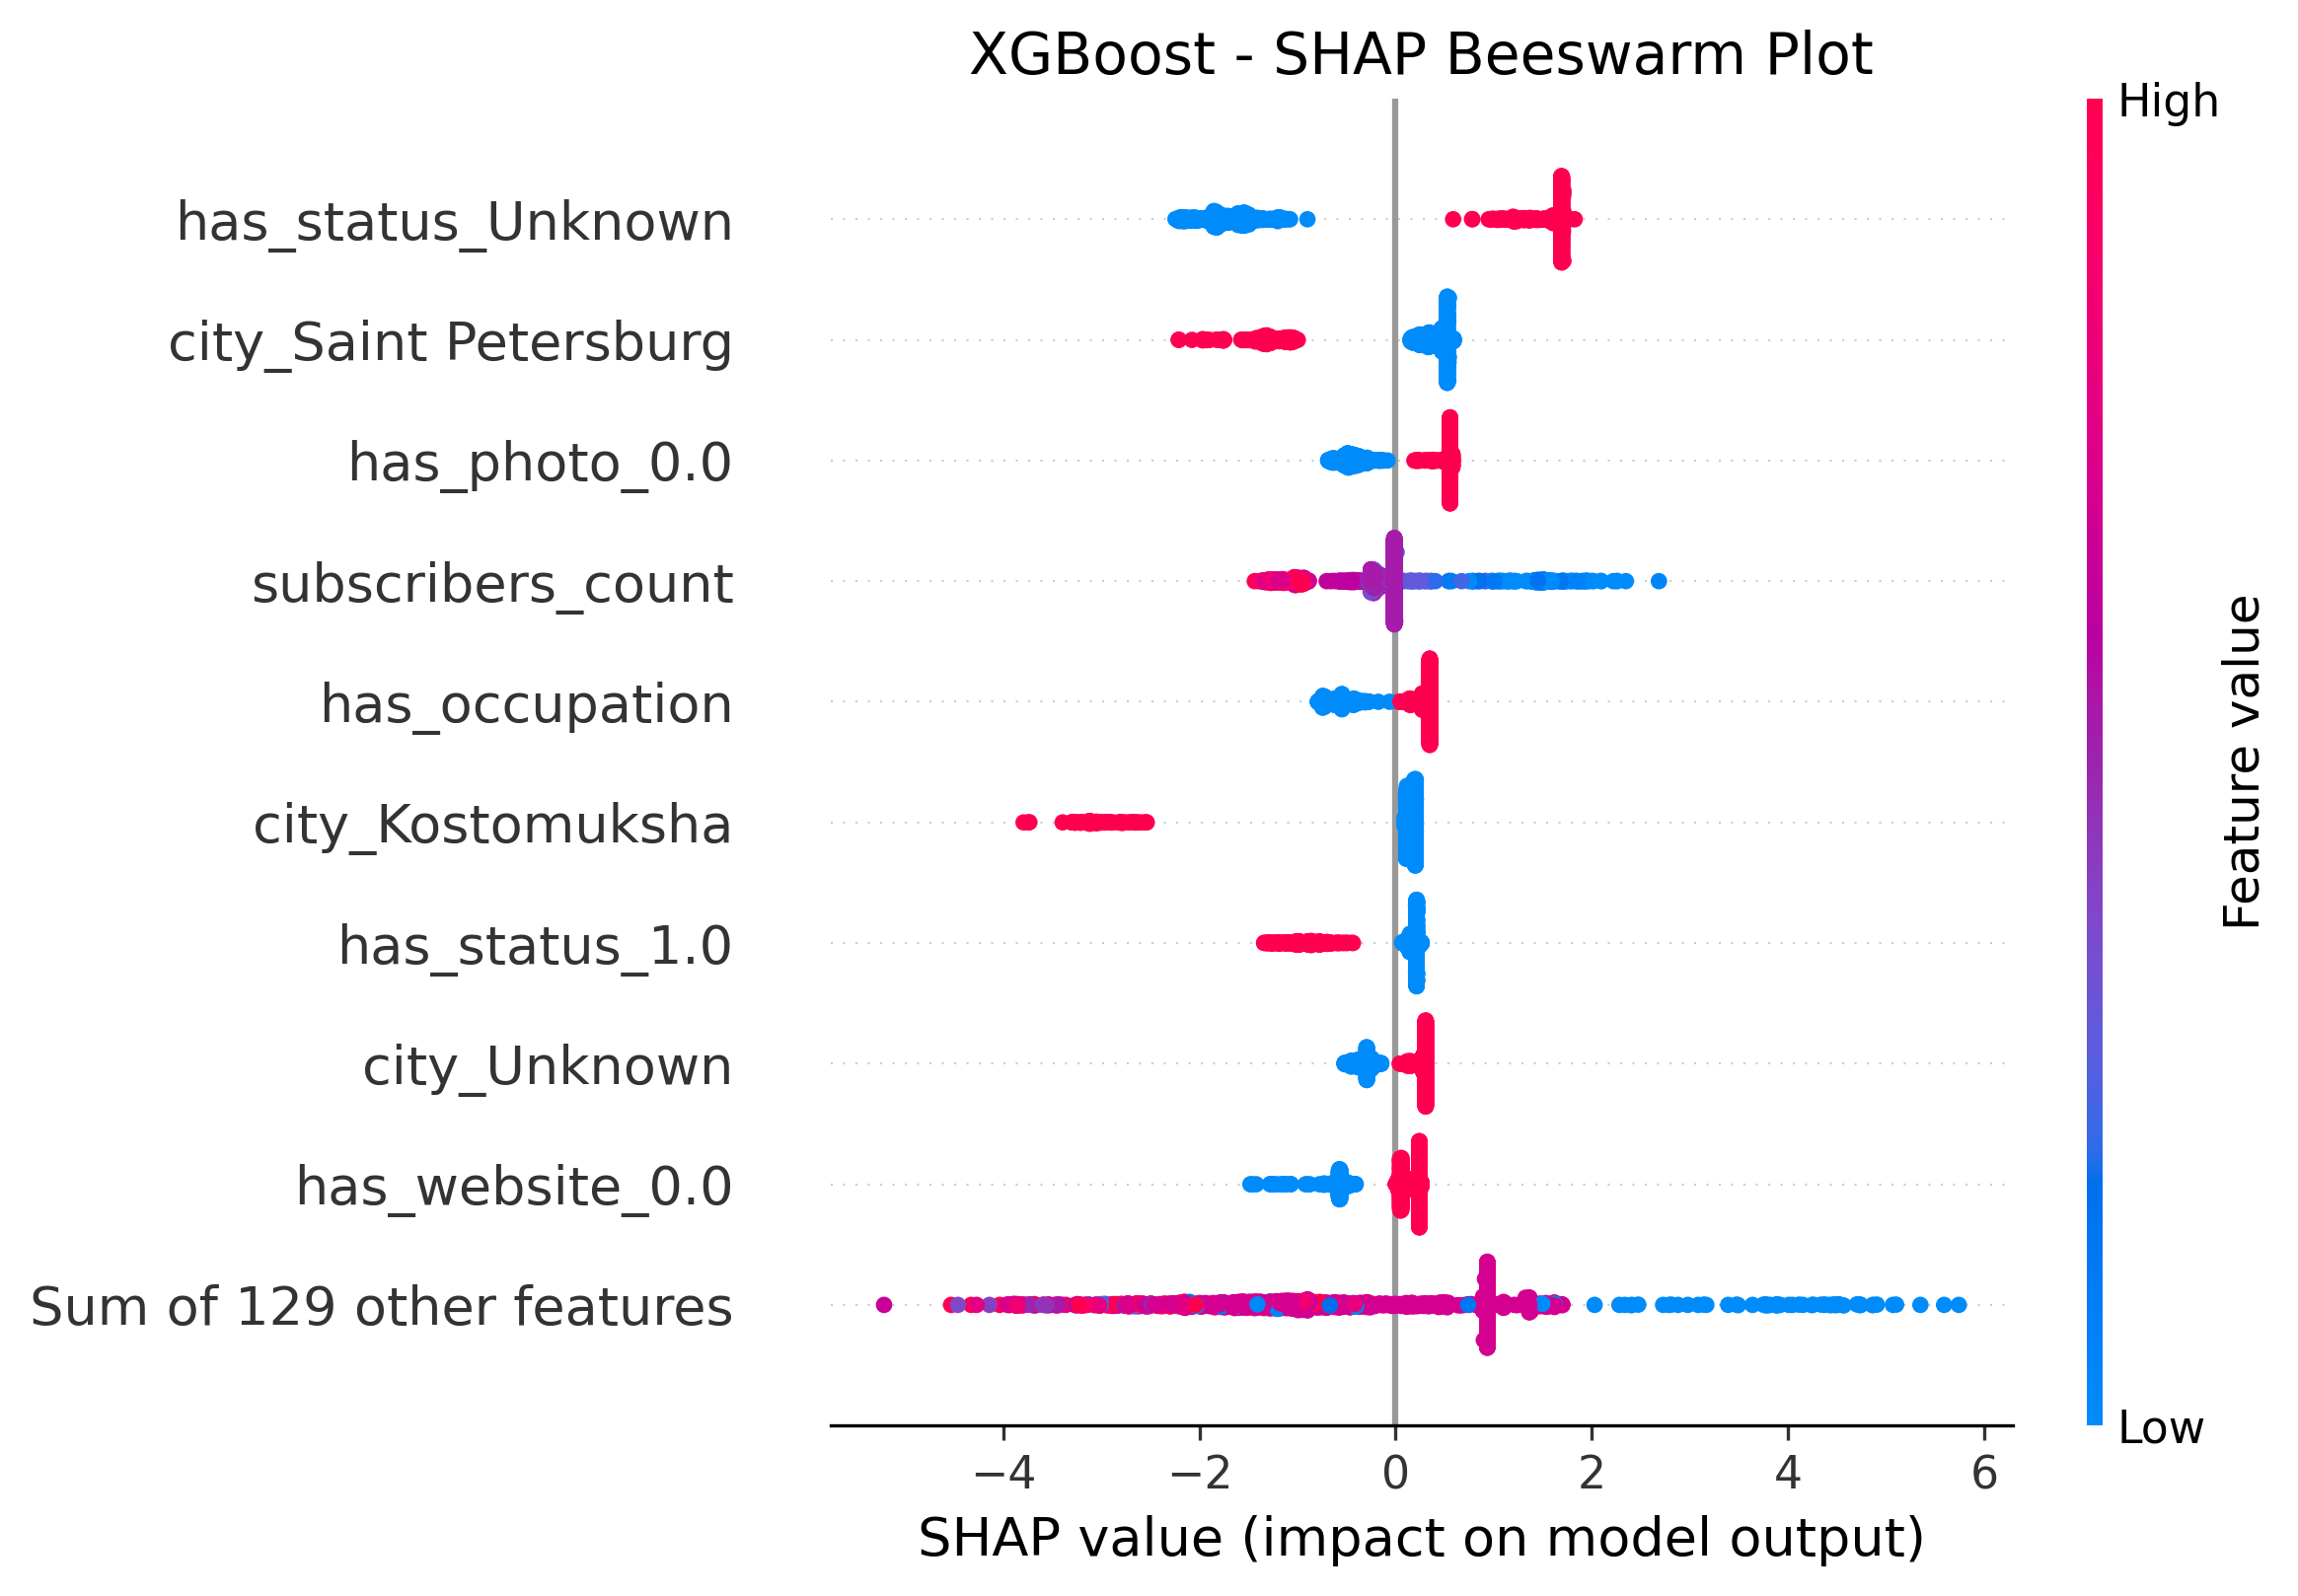
\includegraphics[width=\linewidth]{Figures/xgb_shap_beeswarm.png}
    \caption{SHAP beeswarm plot showing the global feature importance of the trained logistic regression model. Each dot represents a SHAP value for a single prediction and feature. The horizontal position indicates the impact on the model output (positive values push the prediction toward the bot class), while the color reflects the original feature value (red = high, blue = low). Features are sorted top-to-bottom by overall importance.}
    \label{fig:xgb_shap_bee}
\end{figure}


\end{document}